%  --------------------------------------------------------------------------
%  IPA Wochenplaner Dokumentation
%  Created by Marius Küng on 2012-03-12.
%  --------------------------------------------------------------------------

%  --------------------------------------------------------------------------
%  Latex Document Settings
%  --------------------------------------------------------------------------

\documentclass[
11pt, % Schriftgrösse
a4paper, % A4 Papier
BCOR10mm, % Absoluter Wert der Bindekorrektur, z.B. BCOR1cm
DIV14, % Satzspiegel festlegen siehe
       % http://www.ctex.org/documents/packages/nonstd/koma-script.pdf
footsepline = false, % Trennlinie zwischen Textkörper und Fußzeile
                     % bei normalen Seiten
headsepline, % Trennlinie zwischen Kopfzeile und Textkörper
             % bei normalen Seiten
oneside, % Zweiseitig
openright,
halfparskip, % Europäischer Satz mit Abstand zwischen den Absätzen
abstracton, % inkl. Abstract
listof=totocnumbered, % Abb.- und Tab.verzeichnis im Inhaltsverzeichnis
bibliography=totocnumbered % Lit.zeichnis in Inhaltsverzeichnis aufnehmen
]{scrreprt}

\usepackage[automark]{scrpage2} % Gestaltung von kopf- und Fußzeile
\usepackage[ngerman]{babel}
\usepackage[ngerman]{translator}
\usepackage{tocbasic}
\usepackage[utf8]{inputenc}
\usepackage{lmodern} % Latin Modern
\usepackage[T1]{fontenc}
\usepackage{hyphenat}
\usepackage{ae} % Schöne Schriften für PDF-Dateien

% Tradmark
\def\TTra{\textsuperscript{\texttrademark}}

%1.5 Zeilenabstand
\usepackage[onehalfspacing]{setspace}

% Festlegung des Seitenstils (scrpage2)
\pagestyle{scrheadings}
\clearscrheadfoot
\automark[chapter]{section}

% \lehead{\sffamily\upshape\headmark}
% \cehead{}
% \rehead{}
% \lefoot[\pagemark]{\upshape \pagemark}
% \cefoot{}
% \refoot{}
% \lohead{}
% \cohead{}
\lohead{\sffamily\upshape\headmark}
\lofoot{}
\cofoot[\today]{}
\rofoot[\pagemark]{\scshape \pagemark}

% Surround parts of graphics with box
\usepackage{boxedminipage}

% Package for including code in the document
\usepackage{listings}

% If you want to generate a toc for each chapter (use with book)
\usepackage{minitoc}
\usepackage{longtable}

% Abkürzungsverzeichnis erstellen.
\usepackage[printonlyused]{acronym}

% schöne Tabelle zeichnen
\usepackage{booktabs}
\renewcommand{\arraystretch}{1.4} %Die Zeilenabstände in Tabellen angepasst.

% für variable Breiten
\usepackage{tabularx}

% Durchgestrichener Text
\usepackage[normalem]{ulem} %emphasize weiterhin kursiv

% This is now the recommended way for checking for PDFLaTeX:
\usepackage{ifpdf}

\usepackage{eurosym}

\usepackage{natbib}

\usepackage{paralist}

\usepackage{array,ragged2e}

\usepackage[hyperfootnotes=false]{hyperref}
\hypersetup{
  bookmarks=true,         % show bookmarks bar?
  unicode=true,           % non-Latin characters in Acrobat’s bookmarks
  pdftoolbar=true,        % show Acrobat’s toolbar?
  pdfmenubar=true,        % show Acrobat’s menu?
  pdffitwindow=true,      % window fit to page when opened
  pdfstartview={FitH},    % fits the width of the page to the window
  pdftitle={IPA Dokumentation},   
  pdfauthor={Marius Küng},
  pdfsubject={Dokumentation IPA yatplaner},
  pdfcreator={TeX Live 2009},
  pdfproducer={pdfTeX, Version 3.1415926-1.40.10},
  pdfnewwindow=true,      % links in new window
  colorlinks=true,       % false: boxed links; true: colored links
  linkcolor=blue,          % color of internal links
  citecolor=black,        % color of links to bibliography
  filecolor=magenta,      % color of file links
  urlcolor=cyan          % color of external links
  % linkcolor=black,          % color of internal links
  % citecolor=black,        % color of links to bibliography
  % filecolor=black,      % color of file links
  % urlcolor=black          % color of external links
}

\ifpdf
    \usepackage[pdftex]{graphicx}
\else
    \usepackage{graphicx}
\fi

\makeatletter 
\let\orgdescriptionlabel\descriptionlabel 
\renewcommand*{\descriptionlabel}[1]{% 
  \let\orglabel\label 
  \let\label\@gobble 
  \phantomsection 
  \edef\@currentlabel{#1}% 
  %\edef\@currentlabelname{#1}% 
  \let\label\orglabel 
  \orgdescriptionlabel{#1}% 
} 
\makeatother 

%  --------------------------------------------------------------------------
%  Start Document
%  --------------------------------------------------------------------------
\title{Dokumentation IPA Wochenplaner}

\author{IPA in Applikationsentwicklung\\
    \\
    Auszubildender - Marius Küng\\
	Auftraggeber - allink GmbH\\
    Projektleiter - Silvan Spross\\
    Experte - Antonio Di Luzio\\
    Chefexperte - Hans Riesenmann \\
    Durchführungsort - allink GmbH\\
	\\
	Informatikmittelschule Basel}

\date{13.03. - 26.03.2012}

\begin{document}
    \ifpdf
        \DeclareGraphicsExtensions{.pdf, .jpg, .tif}
    \else
        \DeclareGraphicsExtensions{.eps, .jpg}
    \fi

    \pagenumbering{Alph}
  
    \maketitle

    \pagenumbering{arabic}
  
    \tableofcontents
    
    \part{Umfeld und Ablauf}
        \chapter{Aufgabenstellung}
            \section{Titel der Facharbeit} 
Webapplikation zur Ressourcenplanung von allink.creative
    
\section{Thematik}
Es soll eine Webapplikation mit Django erstellt werden, mit welcher die Geschäftsleitung die Ressourcenplanung der Mitarbeiter vornehmen kann. 
Damit soll eine ältere Webapplikation abgelöst werden.
\section{Klassierung}
    
\begin{itemize}
    \item Applikationsentwicklung OO
    \item UNIX / Linux
    \item andere\_Programmiersprache
\end{itemize}
    
\section{Durchführungsblock}
Startblock 1: 12.03.2012 - 23.04.2012\\
IPA-Durchführung: 12.03.2012 - 23.04.2012\\
Einreichung bis: Montag, 30.01.2012\\
    
\section{Ausgangslage}
Bei allink besteht seit Mitte 2010 ein rudimentäres Ressourcenplanungstool. Zur Entwicklung wurden damals jedoch Technologien verwendet, die heute nicht mehr zur Kernkompetenz von allink zählen. Da dieses Tool jedoch jeden Freitag zur Planung der nächsten Woche verwendet wird, ist es seit längerem überfällig es in die bestehende Managementapplikation zu integrieren.

Dank der übermässig langen Testphase des Prototypen sind nun die Anforderungen an das definitive Tool gut bekannt. Daher soll eine Webapplikation mit Django erstellt werden, mit welcher die Geschäftsleitung von allink.creative die Ressourcenplanung der Mitarbeiter vornehmen kann. Damit soll eine ältere Webapplikation abgelöst werden.
    
\section{Detaillierte Aufgabenstellung}
    
Das bestehende Tool namens \"Yatplaner\" soll als Modul im bestehenden Management Tool namens \"allink.planer\" reimplementiert werden. Dabei soll die Bedienbarkeit verbessert werden. Das Ziel ist es das neue Tool so intuitiv bedienen zu können, dass für die Geschäftsleitung keine Schulung nötig ist. Der Praxistest wird voraussichtlich in der letzten IPA Woche an der Wochenplansitzung durchgeführt.

Nebst der begleitenden IPA Dokumentation, wo unter anderem der Funktionsumfang des bestehenden Tools analysiert wird, wird keine zusätzliche Dokumentation gefordert. Der Funktionsumfang des bestehenden Tools soll vom Lernenden in einer Analysephase aufgenommen werden. Dabei sollen die bestehenden Features als Muss- und mögliche neue Features als Kann-Ziele ausformuliert werden.

Der Quellcode des bestehenden Tools ist unter folgender Adresse einsehbar: \\https://github.com/sspross/yatplaner/tree/rails

\section{Mittel und Methoden}
Folgende Technologien sind zwingend zu verwenden:

\begin{itemize}
    \item  Python 2.6
    \item  Django 1.3
    \item  Piston 2.3
    \item  jQuery 1.8
    \item  HTML5
    \item  CSS3
\end{itemize}

Das Tool soll in folgenden Browsern fehlerfrei funktionieren:

\begin{itemize}
    \item Firefox >= 8
    \item Chrome >= 10
    \item Safari >= 5
\end{itemize}

Der Internet Explorer muss explizit nicht unterstützt werden.
    
\section{Vorkenntnisse}
Dem Lernenden sind alle genannten Technologien bereits bekannt. Seit Beginn seines Praktikums im August 2011 setzt er sich damit auseinander. Gewisse Kombinationen wie z.B. mit jQuery einen AJAX Request zu erstellen, sind jedoch Neuland. 
    
\section{Vorarbeiten}
Es findet keine explizite Vorarbeit statt. 
    
\section{Neue Lerninhalte}
Wie bereits erwähnt sind dem Lernenden alle Technologien bereits bekannt. Jedoch sind gewisse Kombinationen noch nie vom Lernenden selbst angewandt worden. Das Know-how ist bei allink ausreichend vorhanden. Der Lernende kann zudem auf eine Vielzahl von bestehenden Projekten zurückgreifen, wo er unzählige Beispiele studieren kann. 
    
\section{Arbeiten in den letzten 6 Monaten}
Der Lernende hat überwiegend Webseiten mit den oben genannten Technologien umgesetzt. Zu seinen umfassendsten Arbeiten zählen bis jetzt eine Webseite eines Immobilienunternehmens und einer Eventplattform eines Finanzkonzerns. Für ersteres arbeitete der Lernende rund 250 Stunden daran. 

        \chapter{Einleitung}
            \section{Projekorganisation}

\begin{figure}[!ht]
\begin{center}
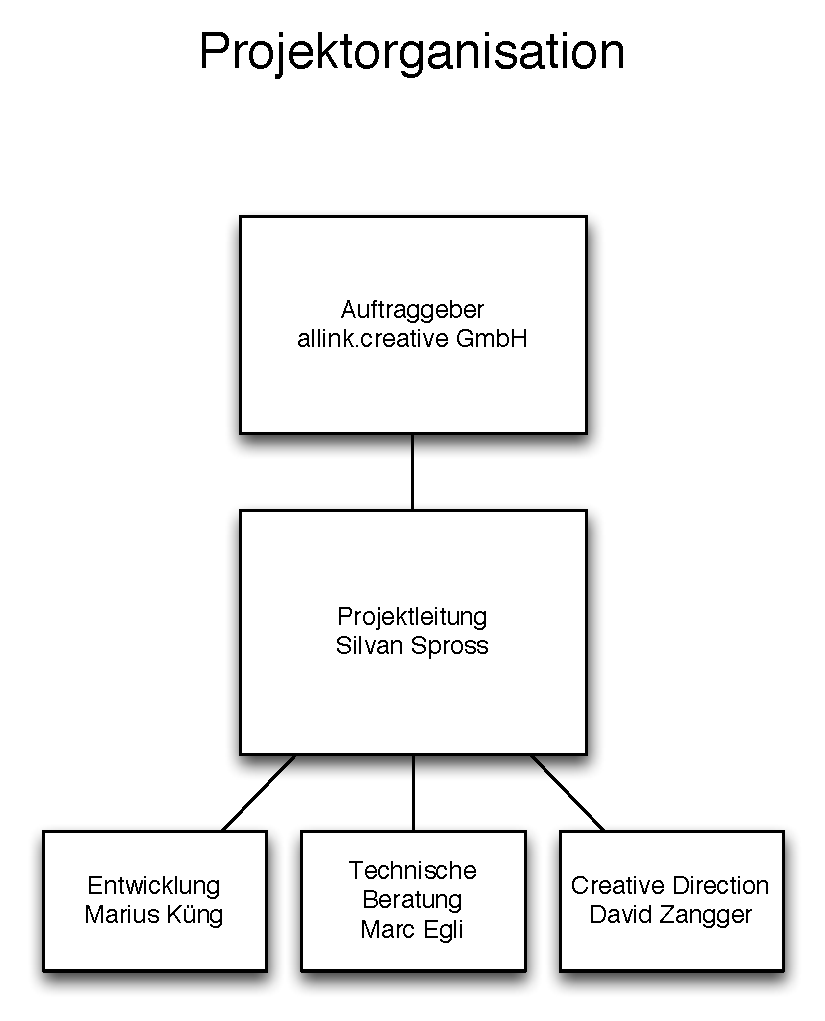
\includegraphics[width=0.5\textwidth,angle=0]{./bilder/01_projektorganisation.pdf}
\caption[Projekorganisation]{Projekorganisation\footnotemark}
\label{pic:01_projektorganisation}
\end{center}
\end{figure}
\footnotetext{Eigene Darstellung}

\section{Vorkenntnisse}

Technologien
\begin{itemize}
    \item Python Grundkenntnisse
    \item Django Fortgeschrittene Kenntnisse
    \item Piston Grundkenntnisse
    \item jQuery Fortgeschrittene Kenntnisse
    \item HTML5 Gute Kenntnisse
    \item CSS3 Gute Kenntnisse
    \item AJAX Fortgeschrittene Kenntnisse
\end{itemize}

Anwendungen
\begin{itemize}
    \item Mehrere komplette Webauftritte realisiert
    \item Applikationen in Django erstellt(News, Blog, Produkteübersicht)
    \item Schnittstellen programmiert (XML, JSON)
    \item Per AJAX dynamische Inhalte laden und einfügen
    \item Dynamische Formulare abschicken und Request entgegenehmen
    \item DOM-Elemente manipulieren, per Events steuern
\end{itemize}
    
\section{Vorarbeiten}
Ich habe, um einen ersten Eindruck über die Funktionalität zu erhalten, den bestehenden yatplaner angeschaut und ausprobiert.
Ausserdem den allink.planer studiert in der, der Wochenplaner implementiert wird.
Ansonsten fand keine explizite Vorarbeit statt.

\section{Firmenstandards}
\begin{itemize}
    \item Betriebsystem: MacOS X
    \item Editor: Textmate
    \item Entwicklungsumgebung: Python Django (Python-Framework für Webapplikationen)
    \item Virtuelle Testumgebung: Django Serversimulation per Terminal steuerbar
    \item Versionierung: Git/Github (Git-Grafik)
    \item Deployment: per fabric auf Apache-Server mit WSGI-Protokoll
\end{itemize}

    \part{Projekt}
        \chapter{Projektbeschreibung}
            %!TEX root = ../dokumentation.tex
\section{Umfeld}
Momentan existiert der Wochenplaner als eigenständige Applikation.
Das Tool fungiert mehr als eine Tafel auf die Post-It's geklebt werden. D. h. die Aufgaben sind nicht direkt im Projektmanagementtool mit der Person verbunden.
Somit bietet das Tool keinen Mehrwert bei der Auswertung des Projektablaufs.\\
\\
Das Tool ist in Ruby on Rails programmiert, was nicht dem Firmenstandard entspricht, und kann deshalb nur mühsam gewartet und erweitert werden.

\section{Präzisierung der Aufgabenstellung}
Die Aufgabenstellung sieht vor, dass mindestens die bestehende Funktionalität vorhanden und die intuitive Bedienung verbessert wird. 
Zur weiteren Präzisierung werde ich eine detaillierte IST-Analyse vornehmen. Diese wird mit dem Auftraggeber besprochen, 
damit die MUSS- und KANN-Ziele erfasst werden können und ersichtlich wird, welche Funktionalität überhaupt noch Sinn machen und was weggelassen werden kann.

\section{Analyse Wochenplaner (IST-Zustand)}

\subsection{Modellierung}
    Analysiert anhand der Rails-Modelle\\
    \\
    Person
    \begin{itemize}
        \item Name
        \item Locked Days (gesperrte Tage, Auswahl von Montag bis Freitag)
        \item Beschreibungstext für jeden gesperrten Tag
    \end{itemize}
    Task
    \begin{itemize}
        \item Name
        \item Datum (Fälligkeitsdatum, DATE)
        \item Person (Fremdschlüssel)
        \item Dauer (Stundenanzahl)
    \end{itemize}

\subsection{Darstellung}
Der Wochenplaner verfügt über mehrere Darstellungen:
\begin{itemize}
    \item Kalenderansicht der aktuellen Woche (siehe Design-Screenshot)
    \item Übersicht aller Angestellten
    \item Monatsansicht pro Person
    \item Übersicht aller erfassten Tasks
\end{itemize}

\subsection{Funktionsumfang}
\begin{itemize}
    \item Neue Task durch Doppelklick auf Personentag per Dialog erfassen
    \item Klick auf Task öffnet die Detailansicht (um bspw. Änderungen vorzunehmen oder die Task zu löschen)
    \item Verschieben eines Tasks per Drag \& Drop
    \begin{itemize}
        \item Task in anderen Tag verschieben
        \item Task einer anderen Person zuweisen
    \end{itemize}
    \item In der Kalenderwoche per Link vor- oder zurückspringen
    \item weitere 7 Tage in der Ansicht anzeigen (funktioniert auch umgekehrt)
    \item Wochentage können für wiederkehrende Events (Schule, Frei) markiert werden
\end{itemize}
\subsection{Defizite}
    \begin{itemize}
        \item Die Sperrtage haben kein Startdatum und sind für jeden Wochentag (Vergangenheit \& Zukunft) erfasst
        \item Die Ajax-Funktionalität beschränkt sich auf Task erstellen und verschieben
        \item Die Bearbeitung der Tasks ist mühsam
    \end{itemize}

\section{Definition Ziele}
In einer Sitzung mit der Projektleitung wurde der IST-Zustand besprochen und die Ziele definiert.
\clearpage
\subsection{MUSS-Ziele}
\begin{table}[!ht]
\begin{center}
    \begin{tabular}{llp{8cm}l}
        \toprule Nr & Funktion & Beschreibung \\
        \midrule 1 & Task erfassen & Der Benutzer kann eine neue Task erfassen. \\
        \midrule 2 & Task Namen geben & Der Benutzer kann einem Task einen Namen geben. \\
        \midrule 3 & Task Datum geben & Der Benutzer kann einem Task ein Datum geben. \\
        \midrule 4 & Task Person zuweisen & Der Benutzer kann einem Task eine Person zuweisen. \\
        \midrule 5 & Task Dauer geben & Der Benutzer kann einem Task eine Dauer (in Stunden) geben. \\
        \midrule 6 & Task bearbeiten & Der Benutzer kann einen Task bearbeiten. \\ 
        \midrule 7 & Task löschen & Der Benutzer kann einen Task löschen. \\
        \midrule 8 & Person hinzufügen & Der Benutzer kann eine Person dem Wochenplaner hinzufügen. \\
        \midrule 9 & Sperrtag Person zuweisen & Der Benutzer kann einer Person einen Sperrtag zuweisen. \\
        \midrule 10 & Sperrtag Namen geben & Der Benutzer kann einem Sperrtag einen Namen geben. \\
        \midrule 11 & Sperrtag bearbeiten & Der Benutzer kann einen Sperrtag bearbeiten.\\
        \midrule 12 & Sperrtag löschen & Der Benutzer kann einen Sperrtag löschen.\\
        \midrule 13 & Task einem Projekt zuweisen & Der Benutzer kann einen Task einem Projekt zuweisen.\\
        \midrule 14 & Person als Partner & Eine Person als Partner kennzeichnen.\\
        \bottomrule
    \end{tabular}
    \caption{Zwingend umzusetzende Funktionen des Prototypen}
    \label{tab:muss_funktionen}
\end{center}
\end{table}
\clearpage
\subsection{KANN-Ziele}
\begin{table}[!ht]
\begin{center}
    \begin{tabular}{llp{6cm}l}
        \toprule Nr & Funktion & Beschreibung & Priorität \\
        \midrule 15 & Task duplizieren & Der Benutzer kann einen Task duplizieren. & 1\\
        \midrule 16 & Sperrtag Startdatum geben & Der Benutzer kann einem Sperrtag ein Start- \& Endatum geben. &  3\\ 
        \midrule 17 & Warnmeldung Max Stunden & Es erscheint eine Warnmeldung wenn die Summe aller Arbeitsstunden pro Tag 8h überschreiten. & 4\\
        \midrule 18 & Tasks sortieren & Tasks können innerhalb eines Tages sortiert werden. & 2\\
        \bottomrule
    \end{tabular}
    \caption{Nicht zwingend umzusetzende Funktionen des Prototypen}
    \label{tab:kann_funktionen}
\end{center}
\end{table}

% \section{Projektmanagement}
% Für dieses Projekt werde ich mich an der Wasserfall-Methode orientieren, da es für den Umfang des Projektes ausreichend ist.

% \section{Lösungsvarianten (SOLL-Möglichkeiten)}
% 
% \section{Entscheidung Projektleitung Variante}
        \chapter{Realisierung}
            %!TEX root = ../dokumentation.tex
\section{ERM allink.planer}
Als Ausgangslage dient mir das ERM des allink.planer. Die Entitäten Person und Project werden mit dem Wochenplaner verknüpft.

\begin{figure}[!ht]
\begin{center}
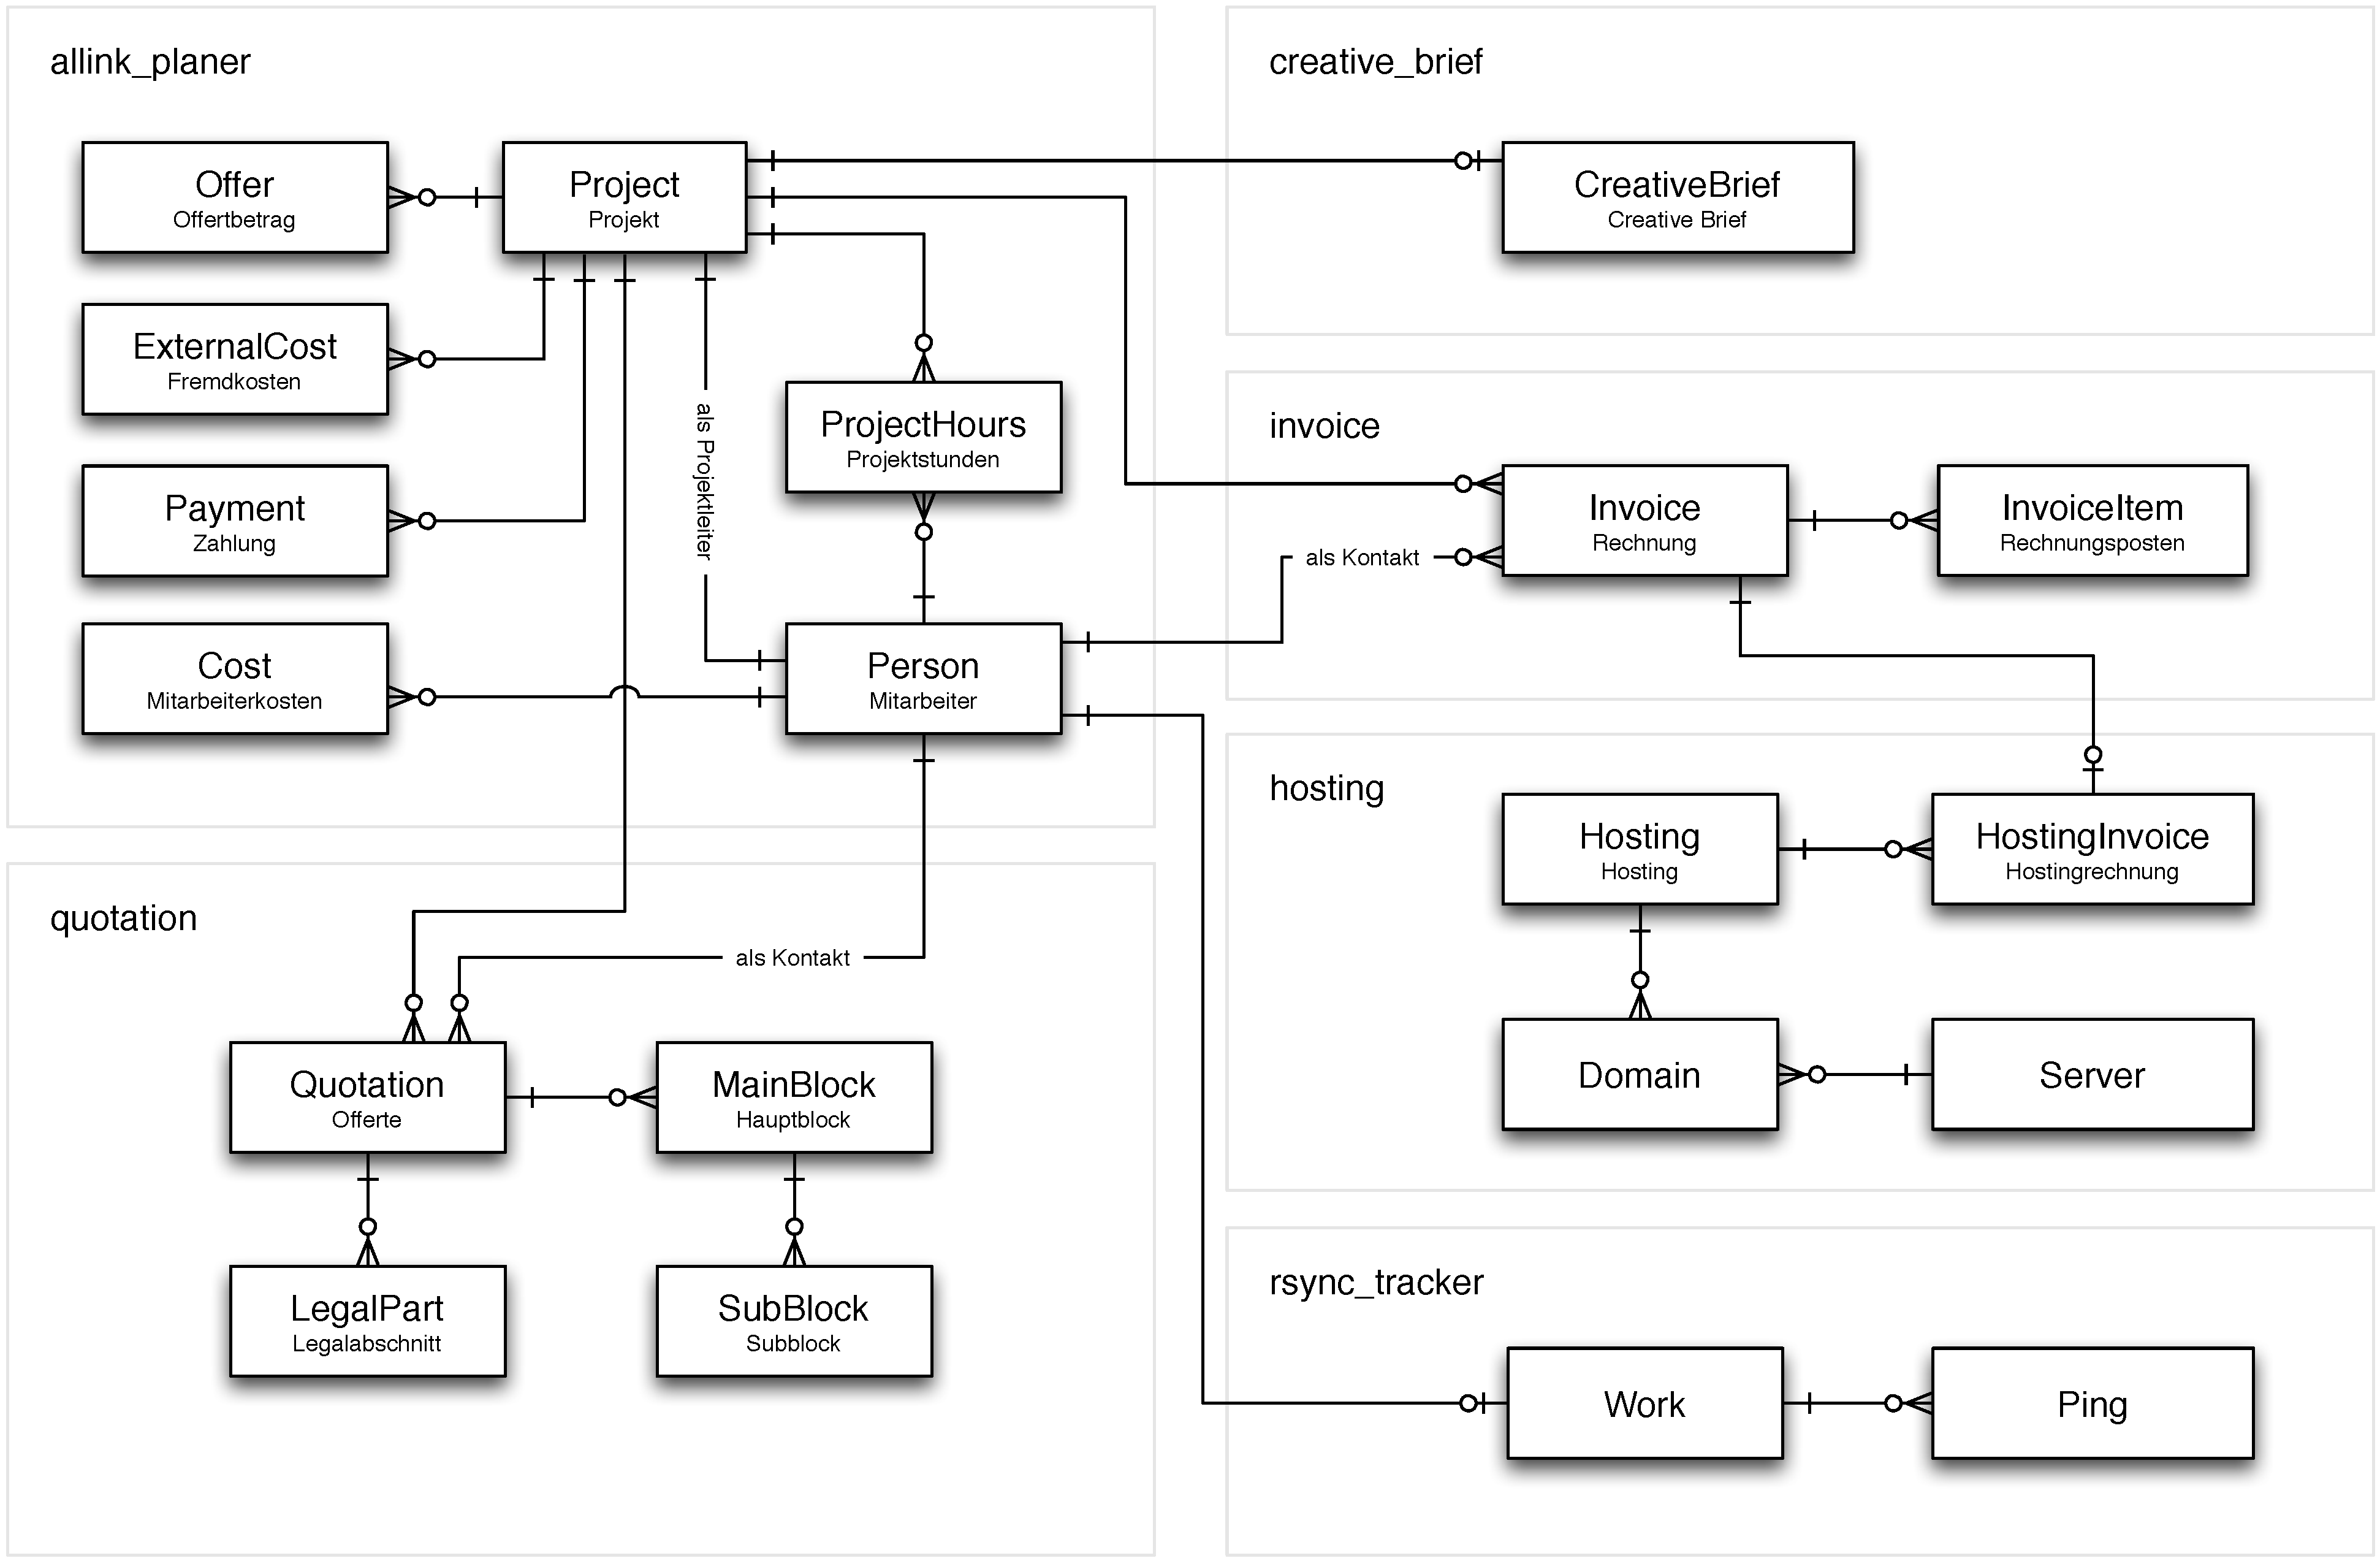
\includegraphics[width=0.99\textwidth,angle=0]{./bilder/erm_planer.pdf}
\caption{ERM allink.planer}
\end{center}
\end{figure}
\footnotetext{Entommen aus allink.planer}

\clearpage

\section{ERM Wochenplaner}
\begin{figure}[!ht]
\begin{center}
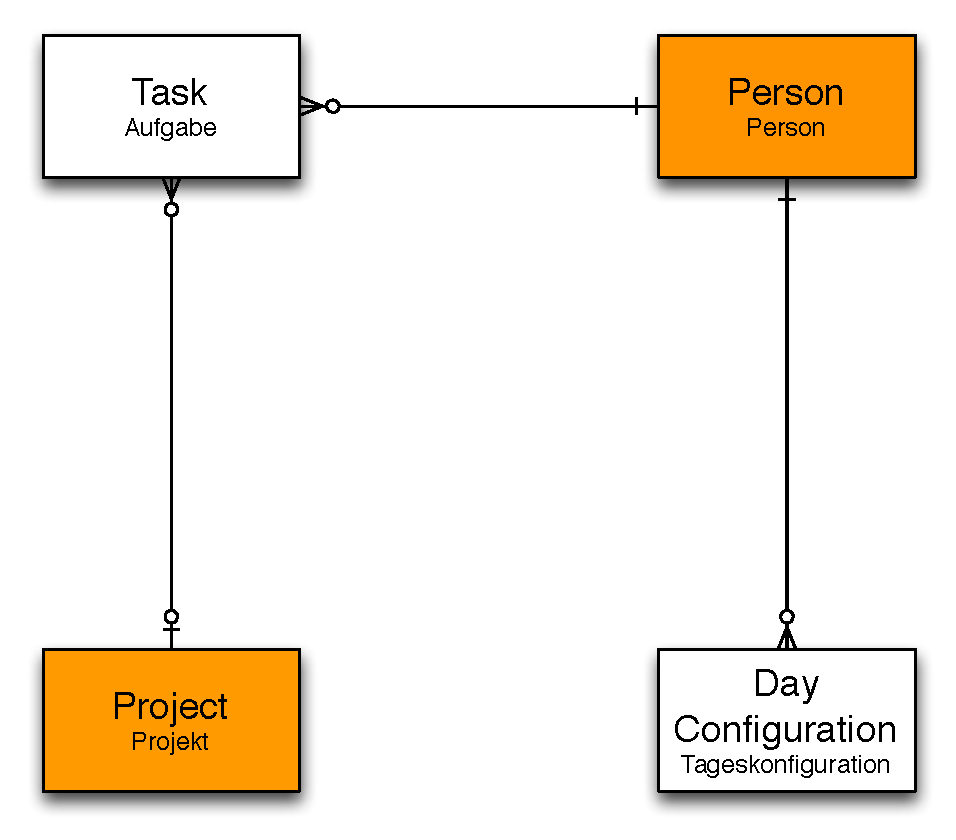
\includegraphics[width=0.99\textwidth,angle=0]{./bilder/erm.pdf}
\caption{ERM Wochenplaner (die Orange hinterlegten Entitäten stammen aus dem allink.planer)}
\end{center}
\end{figure}
\footnotetext{Eigene Darstellung}

\section{Design}
\subsection{Altes Design}
\begin{figure}[!ht]
\begin{center}
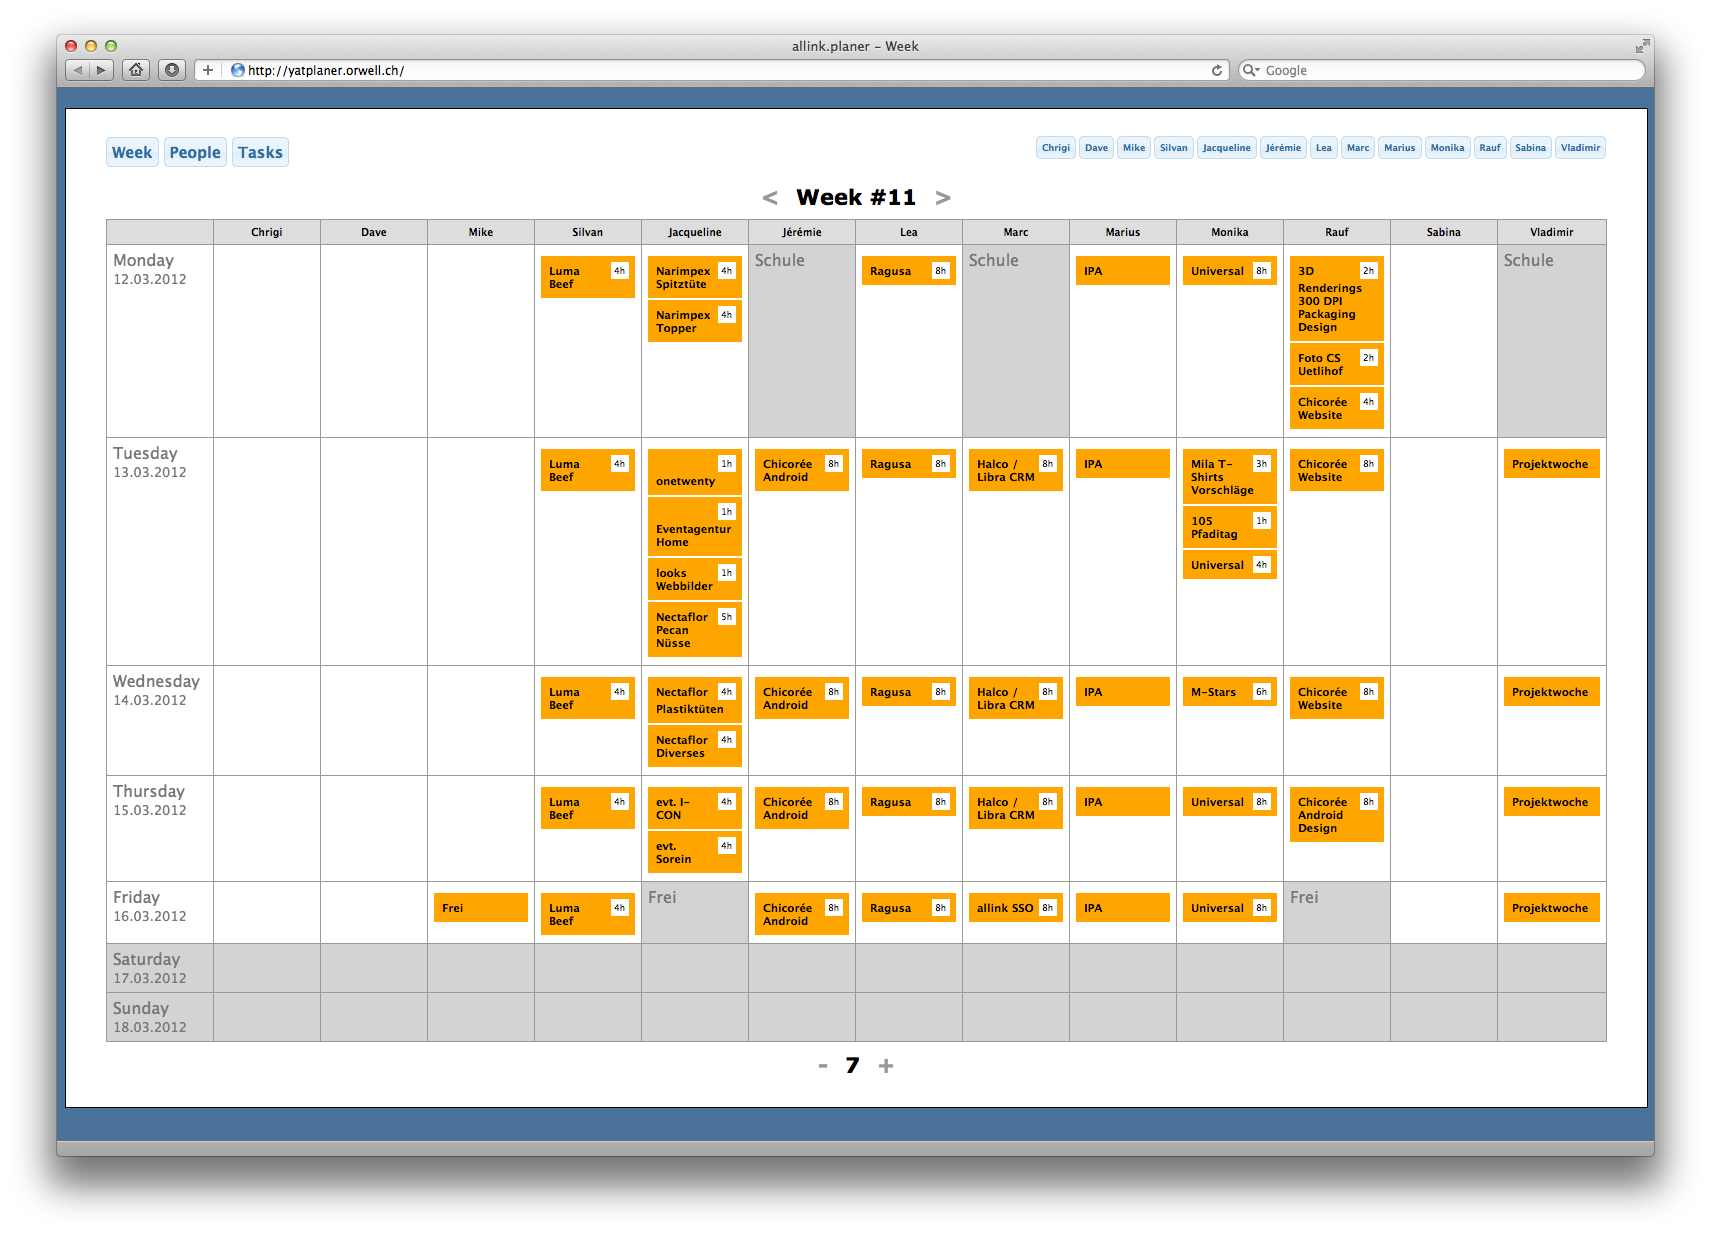
\includegraphics[width=0.99\textwidth,angle=0]{./bilder/yatplaner.png}
\caption{Bisheriges Design des yatplaner}
\end{center}
\end{figure}

\clearpage
\section{Neues Design}
\begin{figure}[!ht]
\begin{center}
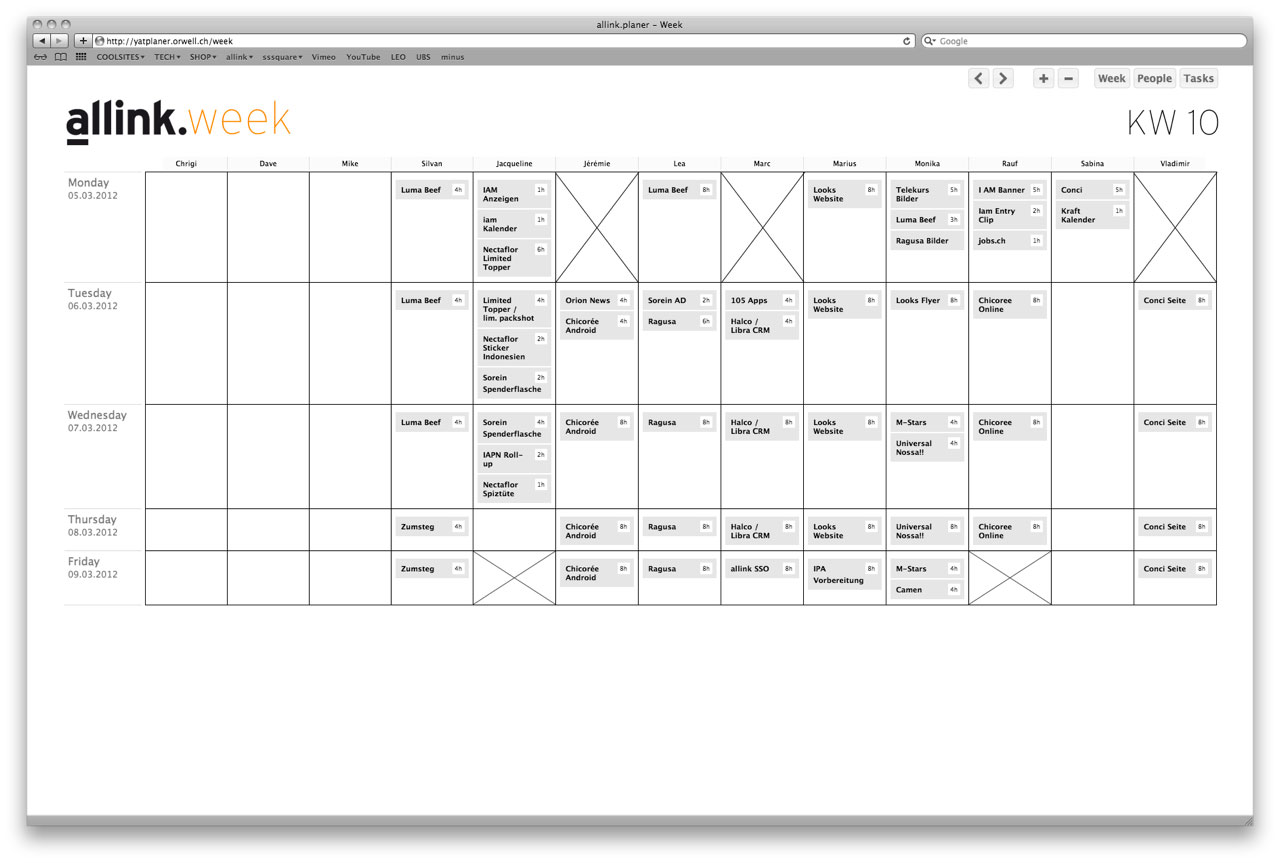
\includegraphics[width=0.99\textwidth,angle=0]{./bilder/wochenplaner.jpg}
\caption{Neues Design}
\end{center}
\end{figure}

%\section{System-Beschreibung}

\section{Modellierung (Django, aufsetzen Projekt) }
\section{Templating Wochenansicht}
\section{JS Funktionalität (CRUD mit jQueryUI \& AJAX) }
\section{Implementierung}
\section{Erreichte Ziele}

        \chapter{Testing}
            %!TEX root = ../dokumentation.tex
\section{Testfälle erfassen}
\section{Testfälle ausführen}
\section{Testbericht (Ziele)}

        \chapter{Konklusion}
            %!TEX root = ../dokumentation.tex
\section{Was ich gelernt habe}
In meiner 10-tägigen IPA habe ich folgendes gelernt:
\begin{itemize}
    \item wie man eine bestehende Applikation analysiert und Muss-/Kann-Ziele erfasst.
    \item planen wie viel Zeit man für eine Aufgabe benötigt
    \item Eine komplexe und datenlastige HTML-Ansicht umzusetzen
    \item Ziele zu definieren und für den zeitlichen Rahmen abzugrenzen
    \item verschachtelte Queries erstellt um eine kompakte Datenabfrage zu generieren
    \item eine dynamische Kommunikation mit dem Server herzustellen
    \item dynamische CRUD-Request erstellen
    \item die jQuery Library jQueryUI anzuwenden
    \item Testfälle erstellen und durchführen
\end{itemize}
\section{Positives}
Ich hatte sehr viel Spass an meiner Arbeit, da es sich um eine Webapplikation handelte die über AJAX CRUD-Funktionalität verfügt und ich etwas derartiges noch nie gemacht habe.
Was mich besonders überraschte war:
\begin{itemize}
    \item in Django Schnittstellen zu programmieren und diese zu erweitern ist relativ simpel.
    \item dass jQuery ohne grössere Probleme einen AJAX-Request bauen und per callback wieder Daten entgegen nehmen kann.
\end{itemize}
Was mich natürlich auch freute war, dass ich alle Ziele erreicht habe, wenn auch nicht unbedingt in der zu Beginn geplanten Umsetzungszeit.
\section{Negatives}
\subsection{Zeitplanung}
Dass ich die Zeitplanung nicht mit einer Timeline umgesetzt habe, machte mich nicht ganz zufrieden.
Jedoch empfand ich es als schwer ein so kleines Projekt so genau planen zu können.\\
Es traten in der Realität immer wieder kleine Probleme auf, die alle zusammen mein Zeitmanagement durcheinander gebracht hätten.
In Zukunft werde ich versuchen Aufgaben besser zu planen damit sie besser mit dem zeitlichen Rahmen übereinstimmen.
\subsection{Testing}
Im Nachhinein wurde mir klar, dass ich meine Testmethode besser von Anfang an in den Programmierprozess hätte einbeziehen sollen oder einen besseren Weg finden, um für diese Funktionalität ein Frontend-Testing durchzuführen.
Ich war der Ansicht, dass die Testmethode für die Testfälle ausreichend ist, da die Realisierung stark auf die Intuitiviät im Frontend ausgerichtet war.
        \chapter{Literaturverzeichnis}
            %!TEX root = ../dokumentation.tex
% python doc
% django doc
% jquery doc
% jqueryui doc
% latex cheat sheet: www.stdout.org/~winston/latex/latexsheet-a4.pdf
% https://docs.djangoproject.com/en/1.3/
% http://wolfram.kriesing.de/blog/index.php/2006/learning-how-to-calculate-with-date-and-time-in-python
% https://github.com/madrobby/keymaster#readme
% http://stackoverflow.com/questions/1771627/preventing-click-event-with-jquery-drag-and-drop
% cloning beispiel http://doctype.com/jqueryui-animate-clone-drop

    \part{Arbeitsjournal}
        \chapter{Arbeitsjournal}
            %!TEX root = ../dokumentation/dokumentation.tex
\section{13.03.2012}
Beginn IPA yatplaner
\begin{itemize}
    \item Dokumentation auf github hosten und versionieren
    \item Kapitelstrukur aufbauen 
    \item Zeitplan erstellen (Planung)
    \item Aufgabenstellung erfassen
    \item Projektorganisation grafisch erfassen
    \item Designbesprechung mit Dave
    \item Vorkenntnisse erfassen
    \item Vorarbeiten erfassen
    \item Firmenstandards erfassen
    \item Ziel erreicht: Teil 1 Der Doku erfasst
    \item Umfeld erfassen
    \item IST-Analyse vorerfassen (Ansichten, Funktionalität)
\end{itemize}
\section{14.03.2012}
\begin{itemize}
    %Teil 2\\
    \item IST-Analyse vorerfassen (Modellierung der Rails App)
    \item Sitzungen mit Silvan Spross und Marc Egli zur Definition der MUSS- und KANN-Ziele
    \item MUSS-Ziele erfasst
    \item KANN-Ziele erfasst
    \item Planung abgeschlossen
    \item ERM für Wochenplaner erstellt
    \item allink.planer github repository gecloned
    \item Entwicklungsumgebung aufgesetzt
    \item Ziel erreicht: Anfang Teil 2 der Dokumentation erfasst und mit Realisierung begonnen
    \item mit Django-Modellierung begonnen (Task, DayConfiguration)
    %\item Habe bis jetzt für Doku mehr Zeit gebraucht als im Zeitplan vorgesehen
\end{itemize}
\section{15.03.2012}
    \begin{itemize}
        \item Kapitel Realisierung weiterführen
        \item Django admin einrichten für week
        \item Testdaten (Personen) in die Entwicklungsumgebung importieren
        \item Problem: Die Wochentage zusammenzufassen war relativ knifflig damit man durch jeden Tag iterieren kann
        \item View erstellen für alle Tasks, Personen und Tage
        \item Template erstellt und Tabelle so aufgesetzt damit Daten korrekt eingefügt werden
        \item Template angefangen zu stylen (CSS)
        \item Ziel erreicht: Daten korrekt aus Modell laden und in Template einsetzen, Template funktioniert
        \item (Bin im Zeitplan mit Realisierung)
    \end{itemize}
\section{16.03.2012}
    \begin{itemize}
        \item Ansicht funktioniert für erste Versuche mit jQueryUI
        \item Task sind verschiebbar und sortierbar in andere Tage (ohne callback/Änderungen werden nicht gespeichert)
        \item alle Tasks werden zu javascript Objekten der Klasse Task
        \item jQuery Methoden hinzugefügt (Click-Events)
        \item Task-Dialog hinzugefügt um neue Task zu erfassen
        \item Task Objekt erweitert mit save Methode wenn eine Task gespeichert wird
        \item Django Task Formular
        \item Django Task Piston Handler (json)
        \item AJAX POST schicken
        \item piston nimmt json-POST entgegen und führt das Formular, aus welches die Daten in die Datenbank speichert
        \item wenn eine neue Task erstellt wurde, wird die neue task.id zurückgeschickt um das neue Javascript Task Objekt abzuspeichern
        \item Ziel erreicht: jQueryUI einrichten, mind. POST per Ajax möglich und dynamisches einfügen in Tabelle
    \end{itemize}
\section{19.03.2012}
    \begin{itemize}
        \item Taskobjekte der aktuellen Woche in javascript dictionary speichern
        \item Hilfestellung Silvan: PUT Funktionalität in Django abhandeln bei existierendem Objekt
        \item Verschieben von Task (PUT Funktionalität)
        \item Klick auf eine Task öffnet Dialog und man kann die Task bearbeiten und abspeichern
        \item Bugfix: wenn man eine Task verschoben wird, öffnet es danach den Bearbeiten-Dialog. Per deaktivieren des click events kann dies behoben werden.
        \item Bugfix: man konnte eine neu erstellte Task nicht verschieben
        \item Projekte werden dynamisch in den Dialog eingefügt und können ausgewählt werden
        \item Task einem Projekt zuweisen
        \item Ziel: PUT Funktionalität erstellen für Task verschieben und ändern
        \item Dokumentation weiter führen
        \item Besprechung mit Silvan Stand IPA
    \end{itemize}
\section{20.03.2012}
    \begin{itemize}
        \item Umsetzung MUSS-Ziele erreicht
        \item Dokumentation weiter geschrieben
        \item feature task duplizieren ausprobiert (Kann-Ziel)
        \item Bugfix: Taskzelle ist zu wenig hoch um problemlos neue Task in Zelle zu verschieben
        \item Bugfix: Bei Bearbeitung einer Task wird aktuelles Projekt nicht mitgeschickt
    \end{itemize}
\section{21.03.2012}
    \begin{itemize}
        \item Sperrtag bild ausgewechselt
        \item Bugfix: wenn man im Template die Woche wechselt kann das Datumsformat nicht vearbeitet werden
        \item Queries optimieren mit Marc, verschachtelte Tuples für queries
        \item Dokumentation weiter geschrieben
        \item Kleinere Optimierungen
        \item Cloning weiter versuchen
    \end{itemize}
\section{22.03.2012}
    \begin{itemize}
        \item Fehlerbehebungen im Template: Kalenderwoche wird nicht aktualisiert
        \item KANN-Ziel Tasks sortieren
        \item KANN-Ziel Warnung wenn Tasks in Tag mehr als 8h Stunden betragen
        \item KANN-Ziel Einer Tageskonfiguration ein Startdatum setzen
        \item Bugfix wenn neue Task erstellt wurde konnte sie nicht direkt bearbeitet werden.
        \item Besprechung Sperrtage habe ein Start- und Enddatum und können von weiteren Sperrtagen ersetzt ohne aus der DB gelöscht zu werden
        \item Mit Unterstützung von Marc die beste Lösung finden die Sperrtage auszulesen (Bei jedem Tag abfragen)
        \item Bugfix man kann nicht weniger als 1 Woche anzeigen
        \item Bugfix wenn man die Tagesanzahl erhöht wird aktuelles Datum nicht berücksichtigt
        \item Besprechung wie das Task-cloning am besten implementiert wird
    \end{itemize}
\section{23.03.2012}
    \begin{itemize}
        \item Task kann per Klick dupliziert werden (es wird eine neue mit gleichem Inhalt erzeugt und unten eingefügt)
        \item Task kann per Klick gelöscht werden
        \item Doku schreiben
        \item Mit Silvan Wochenplaner angeschaut und Darstellungsanpassungen vorgenommen
        \item Abnahme Wochenplaner Silvan
    \end{itemize}
\section{26.03.2012}
    \begin{itemize}
        \item Bugfix bei verschieben von Task auf max. Stunden Anzahl prüfen.
        \item Bugfix wenn bei neuem Task keine Stunden angegeben sind.
        \item Dokumentation überarbeiten
        \item Dokumentation fertigstellen
        \item IPA Dokumentation einreichen
    \end{itemize}
    
    \listoffigures
    \listoftables
    % \lstlistoflistings
  
    \bibliographystyle{unsrtnat}
    \bibliography{literaturverzeichnis}
        
\end{document}
